\chapter{Experiment research on solar thermal power system}

In Chapter~\ref{cha:Modeling}, MATLAB is used as the simulation tool to develop the models of the key components of solar thermal systems. Based on these component models, the cascade system model was developed.
The mechanism of trough collector was studied. Under the condition of assumption of uniform overall heat transfer coefficient, the correlations between temperature rise, mass flow of the HTF, solar direct normal irradiance, ambient temperature and other factors were derived. The theoretical formula of the efficiency of trough collector was obtained.
The heat losses of dish collector were analyzed in detail. A thermal network model of the dish receiver was established. Using classical heat transfer correlations, each temperature node of the heat network was solved and the thermal efficiency of the dish collector was obtained.
%For organic Rankine cycle (ORC) system, processes of the Rankine cycle were analyzed and the Rankine cycle efficiency formula was derived.

To understand the solar thermal power generation system more deeply and to validate the applicable range and error of the proposed component models, a platform includes trough concentrating collector, dish concentrating collector and ORC system was built in Wuhan. The construction of this solar thermal platform provides a good foundation for future cascade solar power generation system.

\section{Platform introduction}

\begin{figure}[!ht]
\centering
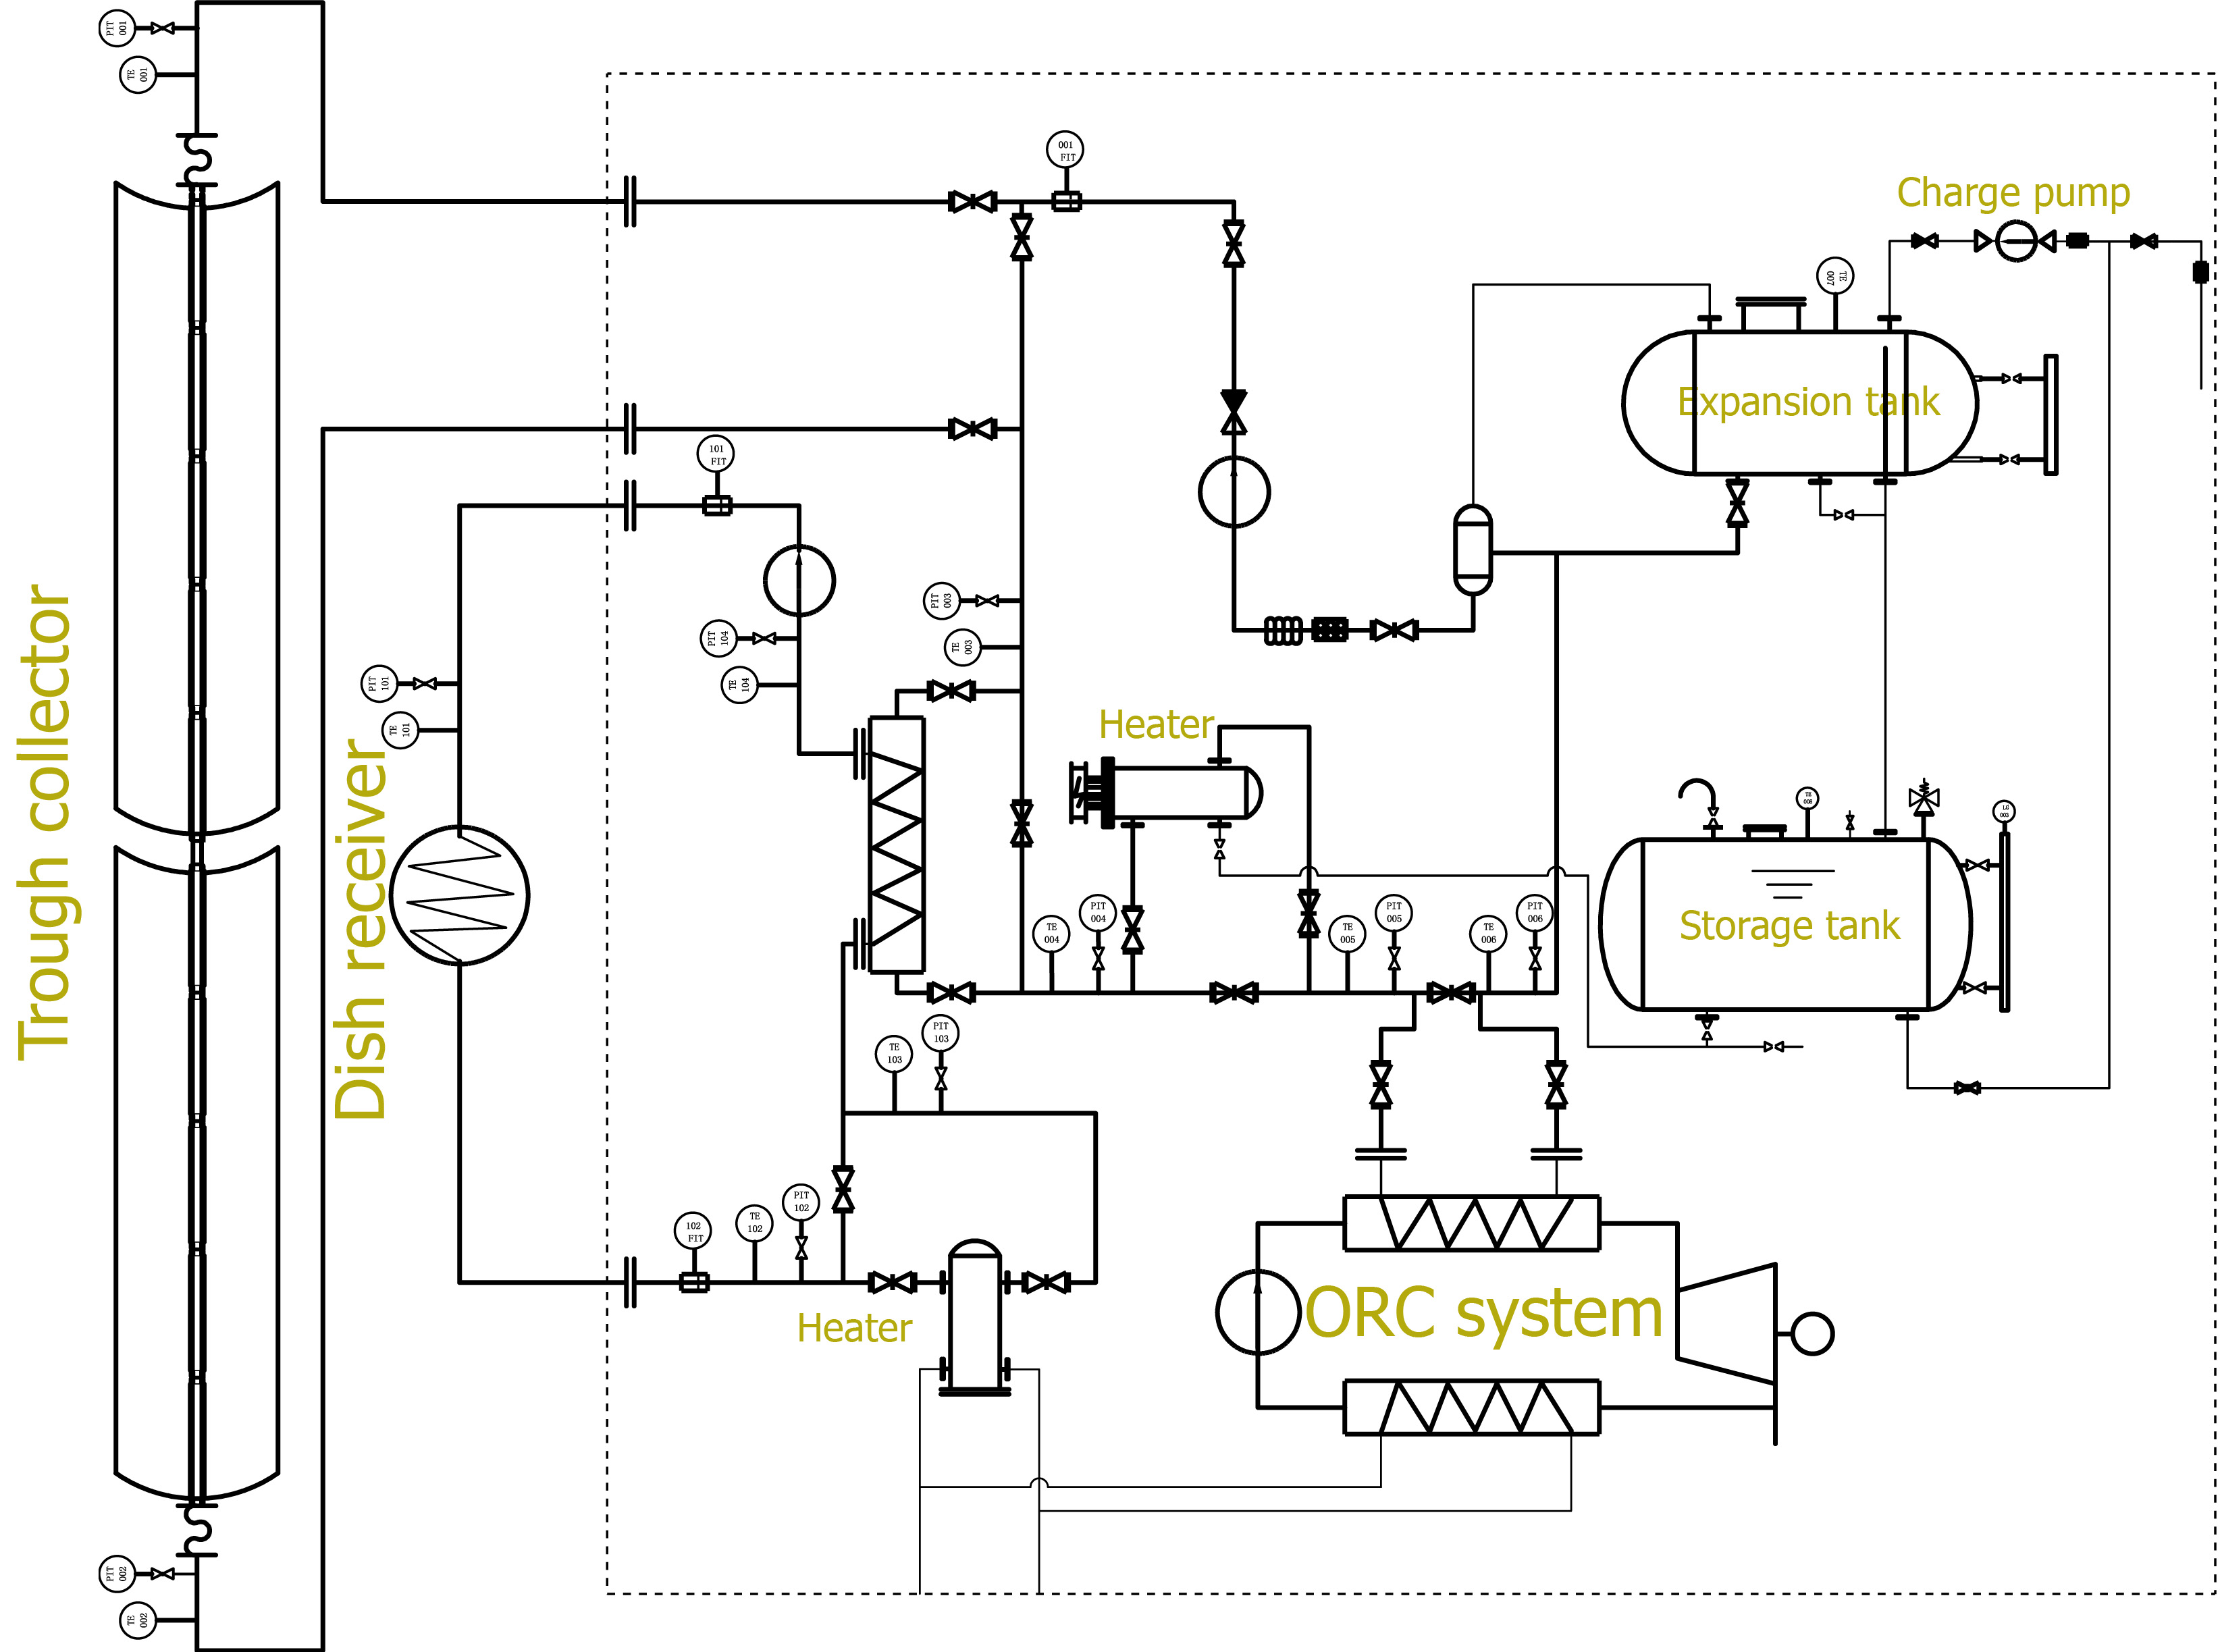
\includegraphics[width=1.0\textwidth]{fig/platform.jpg}
\caption{Schematic structure of the platform}\label{fig:platform}
\end{figure}
Figure~\ref{fig:platform} shows the schematic structure of the solar thermal power platform. 
Three circuits, the air circuit, oil circuit and organic fluid circuit, are created by different fluids. In the air circuit, air in the environment is first compressed in the compressor, and warmed by a heater, 
then heated in dish receiver, then flows into the air-oil heat exchanger to provide heat for Rankine cycle and finally through the water cooling system back to the environment. 
In the oil circuit, the oil is first heated in the trough collector and then flows into the air-oil heat exchanger to obtain the heat provided by the air. The heated oil flows 
into the evaporator of the ORC system to provide heat for the ORC system, then through the pump back to the trough collector.
In the organic fluid circuit, the organic fluid first absorbs the heat provided by the oil in the evaporator, then flows into the ORC turbine for expansion. After expansion, the organic fluid flows into the regenerator to recover part of the overheating heat, then into the condenser, and back to the regenerator to reuse the rejected heat, then through the pump back to the evaporator.

The following describes key components of the platform.

\subsection{Trough collector}
The trough collector is east-west oriented due to land constrains. It is made of parabolic reflector, receiver and bracket. Figure~\ref{fig:TroughCollector} shows the photo of the trough collector. The reflector is 20$\,\mathrm{m}$ long, and 2.55$\,\mathrm{m}$ wide. It consists of a glass tube and a metal black pipe, vacuum is maintained between the two to reduce heat loss. 
The external diameter of the glass tube is 0.11$\,\mathrm{m}$, and the internal diameter is 0.106$\,\mathrm{m}$.
The external diameter of the metal tube is 0.038$\,\mathrm{m}$, and the internal diameter is 0.035$\,\mathrm{m}$.
The bracket is applied to support the reflector and receiver. Its structure is safe enough to resist common windy, stormy and snowy weather conditions. The mechanical structures for rotation, positioning and connection are simple and reliable, easy for mounting, dismounting and transportation, and convenient for operation and maintenance.
Single-axis tracking system is applied for the trough collector system. The program algorithm is used for real-time automatic tracking with small tracking error. Manual mode is also an optional choice. The buttons in the control cabinet make it convenient to adjust the collector to a desired direction. In addition, it provides automatic protection and manual operation protection in case of emergency.

SINOPEC L-QD350 synthetic thermal oil is applied as the HTF of the trough collector system. Its typical physical parameters are provided from the seller.

\begin{figure}[!ht]
\centering
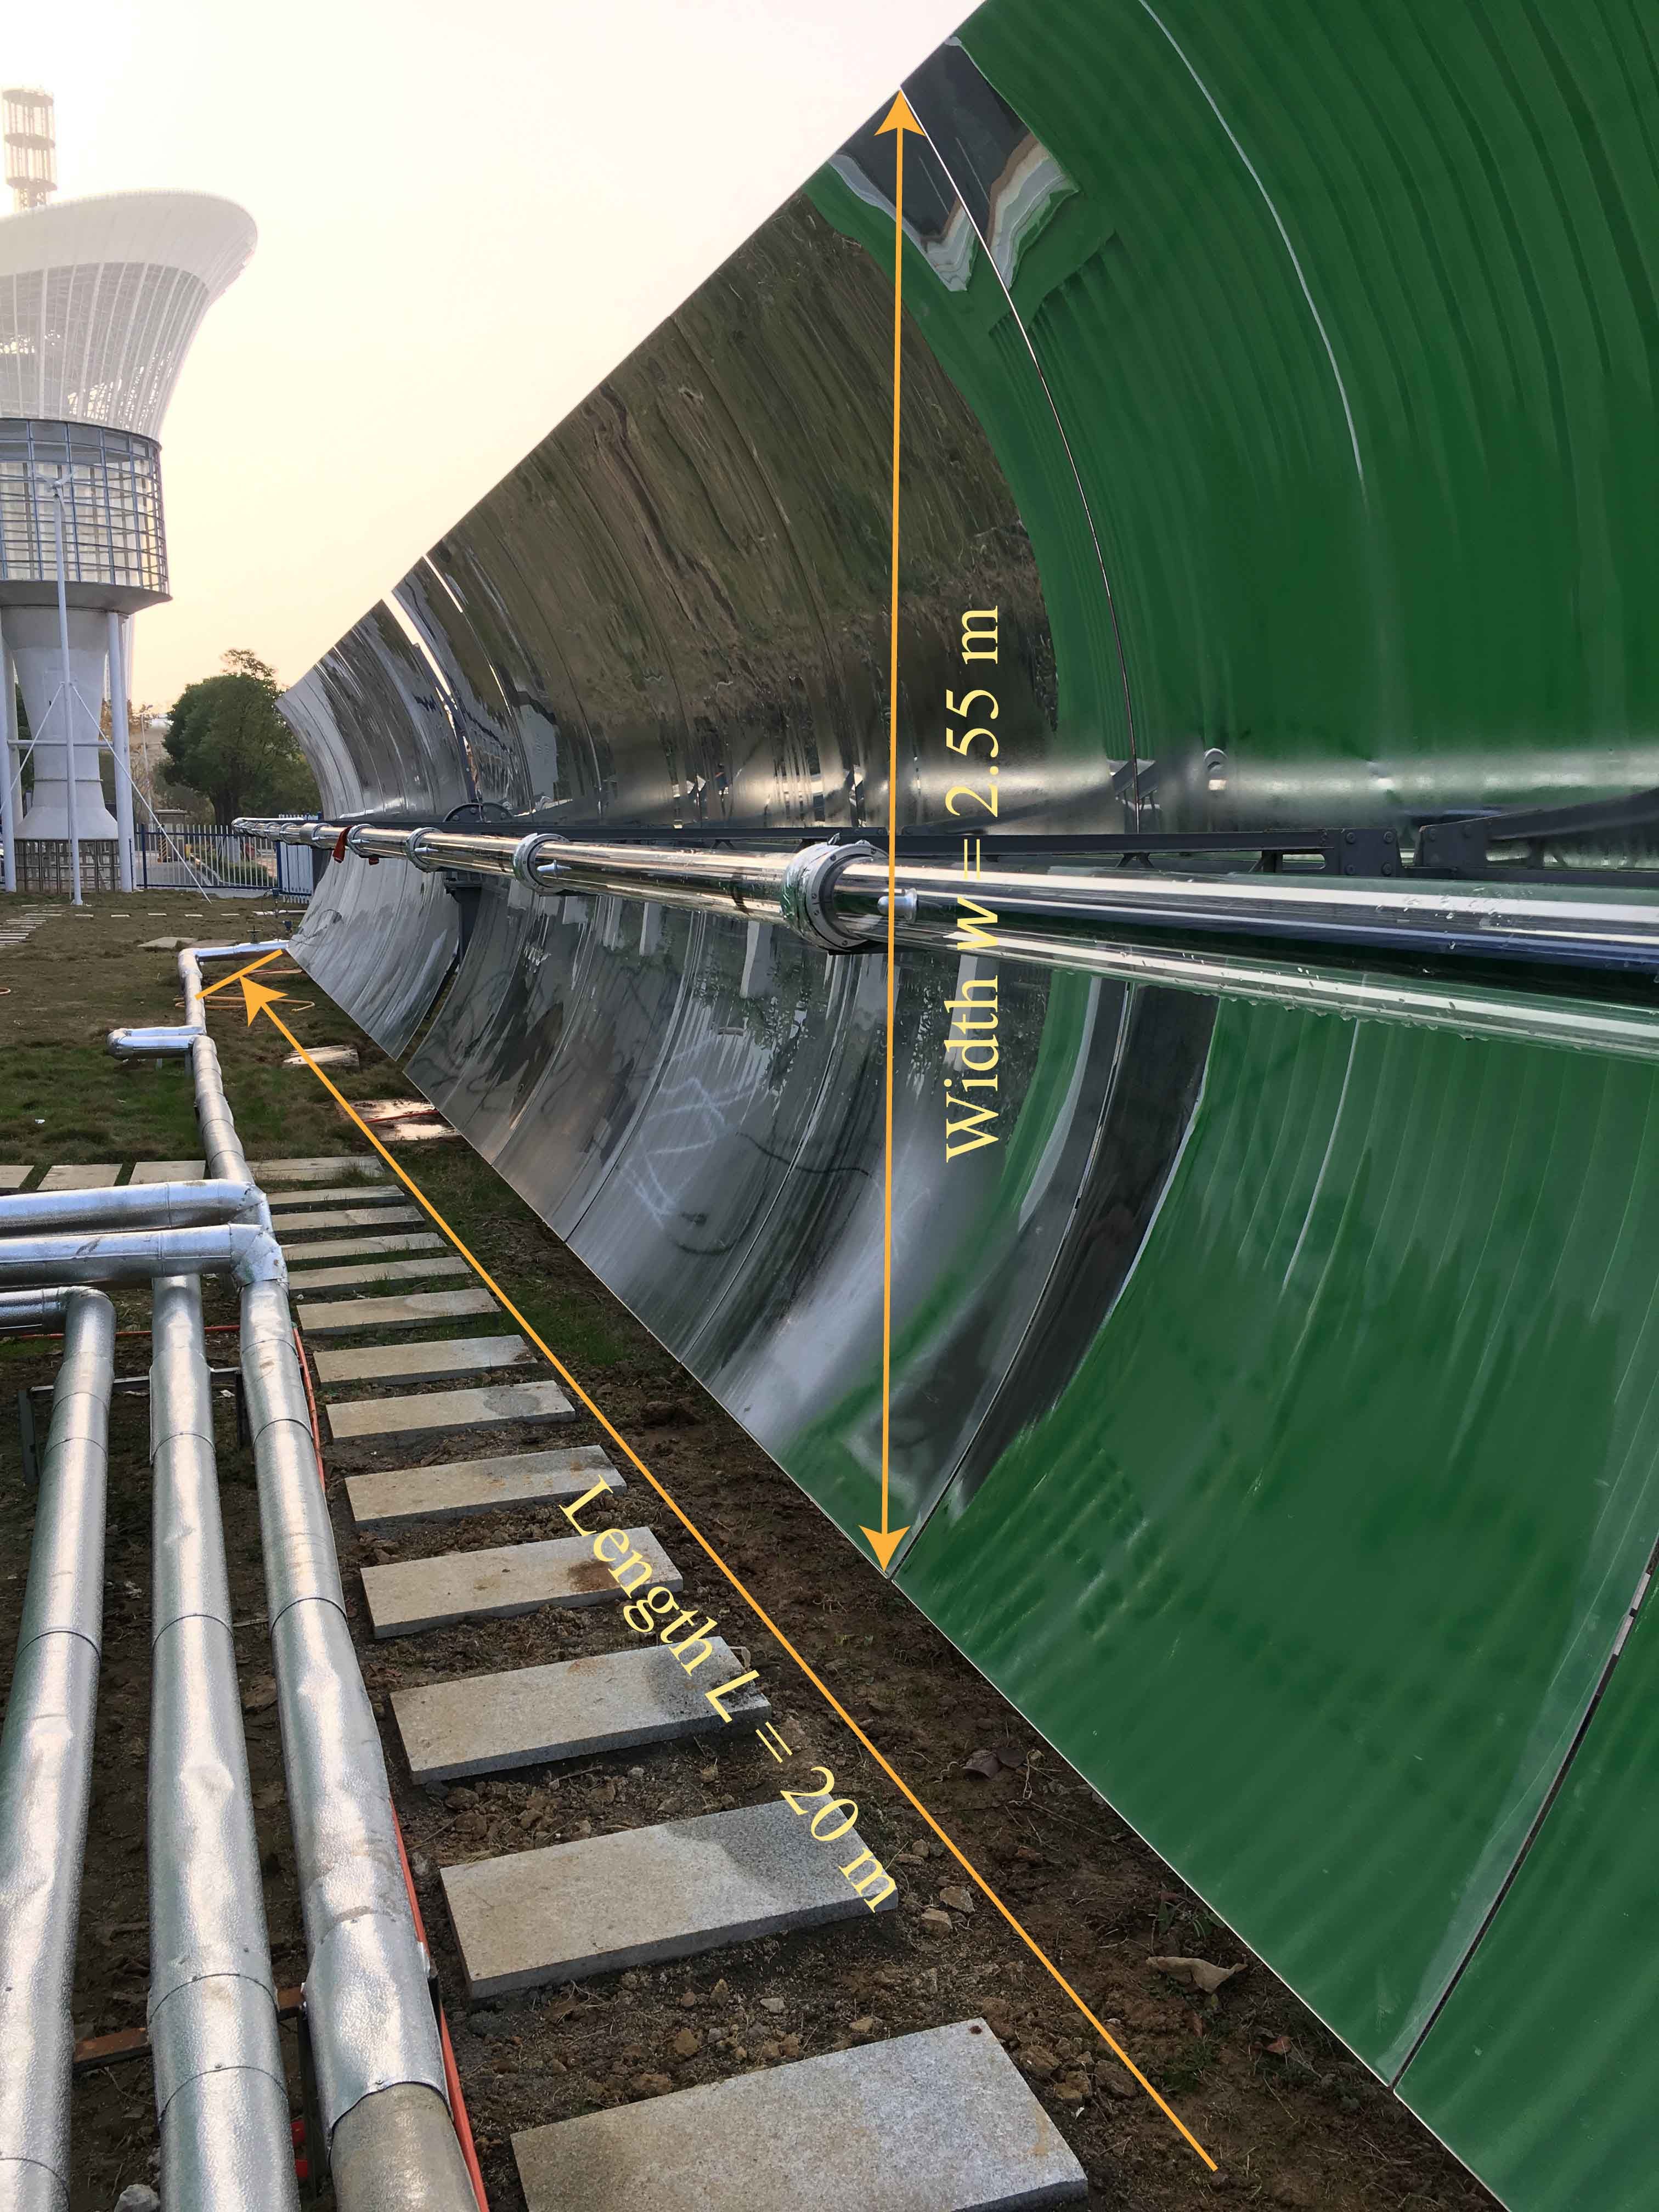
\includegraphics[width=0.7\textwidth]{fig/TroughCollector.jpg}
\caption{Trough collector of the platform}\label{fig:TroughCollector}
\end{figure}

\subsection{Dish collector}

\begin{figure}[!ht]
\centering
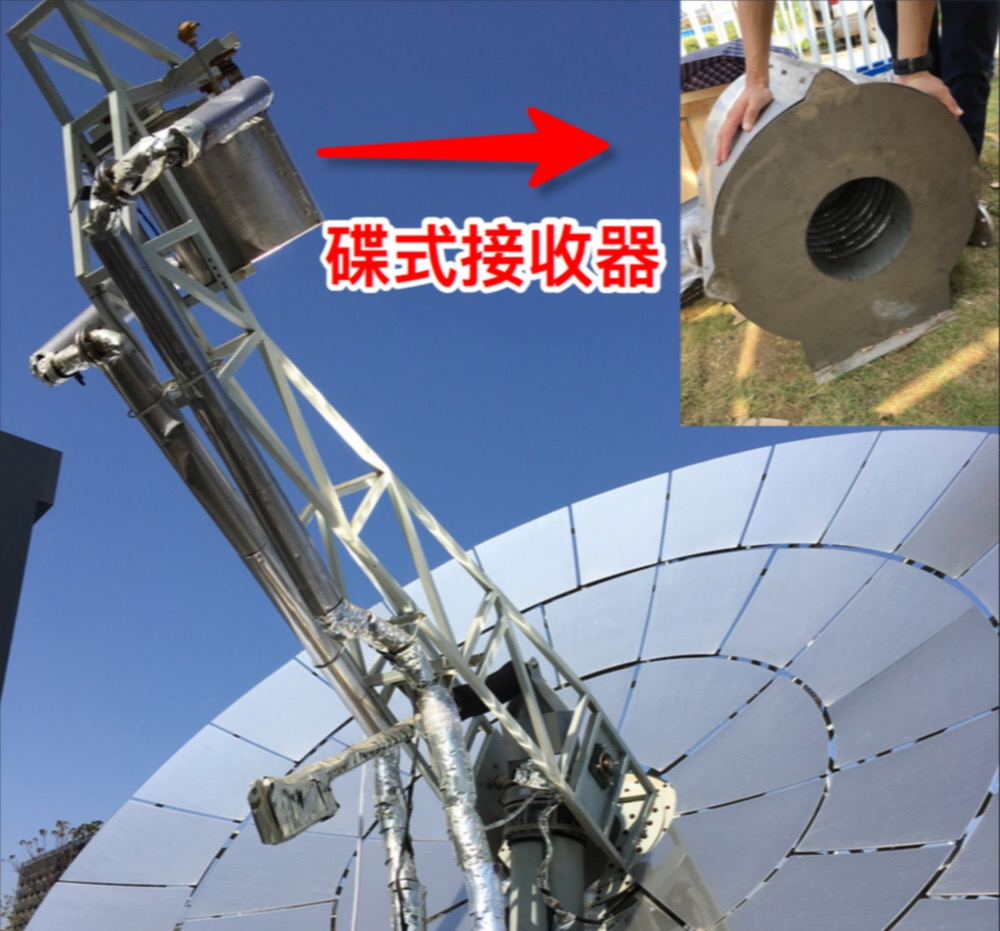
\includegraphics[width=0.7\textwidth]{fig/DishCollector.jpg}
\caption{Dish collector of the platform}\label{fig:DishCollector}
\end{figure}
Figure~\ref{fig:DishCollector} shows the photo of the dish collector. The reflector is made of multiple curved mirrors. When the aperture is facing to the sun, each of the mirrors reflects the sunlight to the focal point. 
%A notch was designed for rotating the collector. When calculating the effective area of the reflector
A self-designed receiver is mounted at the focal point of the dish reflector, as shown at top of the photo in Figure~\ref{fig:DishCollector}.
The key parameters of the dish collector are listed in Table~\ref{tab:ddc}. 
\begin{table}[htbp]
	\caption{Key parameters of the designed dish collector}
	\begin{center}
	\begin{tabular}{cccccc}
		\toprule
		Parameter		&	Value	&	Parameter		&	Value	&	Parameter		&	Value\\
		\midrule
		$d_{cav}$	&	0.45$\,\mathrm{m}$	&	$\epsilon_{insu}$	&	0.6	&	$\theta_{dc}$	&	20$^\circ$\\
		$\delta_{insu}$	&	0.11$\,\mathrm{m}$	&	$\alpha_{cav}$	&	0.87	&	$\gamma$	&	0.97\\
		$dep_{cav}$	&	0.45$\,\mathrm{m}$	&	$\delta_a$		&	0.002$\,\mathrm{m}$	&	$\eta_{shading}$	&	1\\
		$d_{ap}$	&	0.25$\,\mathrm{m}$	&	$d_{i,1}$	&	0.07$\,\mathrm{m}$	&	$\rho$	&	0.91\\
		$\lambda_{insu}$	&	0.06$\,\mathrm{W/(m\cdot K)}$	&	$A_{dc}$	&	23.3$\,\mathrm{m^2}$	&	\\		
		\bottomrule
	\end{tabular}
	\end{center}
	\label{tab:ddc}
\end{table}

The YYGN-GR-1A automatic two-axis tracking control system is used for the dish collector system. Both algorithm tracking method and sensor tracking method are applied for the tracking system. Usually, at the beginning of the focusing process, manual mode is applied to roughly rotate the collector towards the sun. Then switch to the automatic mode to precisely face to the sun. And the algorithm tracking method will take over and keep tracking the sun. This provides a more reliable tracking system with tracking error of less than 0.2$^\circ$ without cumulative error.
The control cabinet of the dish collector provides mechanical, electrical and other optional controls. It also monitors the wind speed and provides the function of set maximum wind speed for safety. When the wind is too strong, it will rotate the collector to a safe angle (facing the zenith).

\subsection{ORC system}
Hot oil (heated by the trough collector and/or the heater) is supplied to the ORC system. 
In the hot loop, input temperature of the supplied oil is 180$\mathrm{^\circ C}$, and output temperature is 160$\mathrm{^\circ C}$. Flow rate of 0.44$\,\mathrm{kg/s}$ is required to reach the nominal output gross power 1.5$\,\mathrm{kW}$. In the cold loop, input temperature of tap water is 30$\mathrm{^\circ C}$, and output temperature is 37$\mathrm{^\circ C}$. The water flow rate is about 0.83$\,\mathrm{kg/s}$.

\begin{figure}[!ht]
\centering
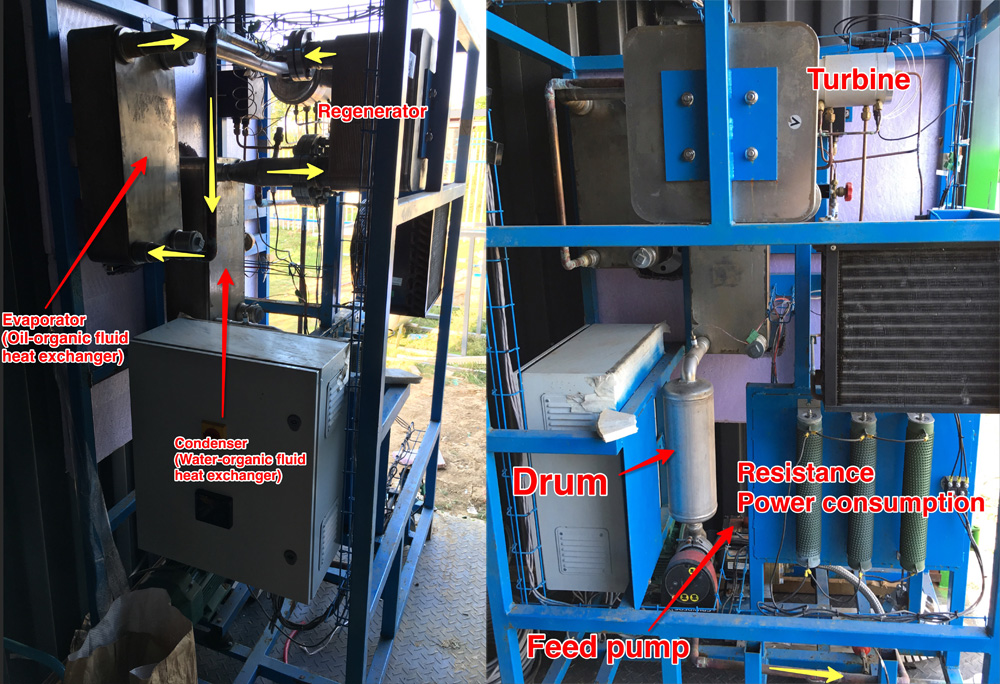
\includegraphics[width=0.7\textwidth]{fig/ORCsystem.jpg}
\caption{ORC system of the platform}\label{fig:ORCsystem}
\end{figure}
Figure~\ref{fig:ORCsystem} shows photos of the ORC system. It is made of evaporator, high speed ORC turbine, generator, regenerator, condenser, organic working medium pump, electrical control cabinet and the connection pipes.

The control cabinet provide a touch screen to control the ORC system. Both automatic mode and manual mode are provided. In automatic mode, all the start up work and shut down work will be completed by procedure automatically. In manual mode, you can manually set the parameters such as the speed of the organic fluid pump to provide precise control of the system.

\begin{figure}[!ht]
\centering
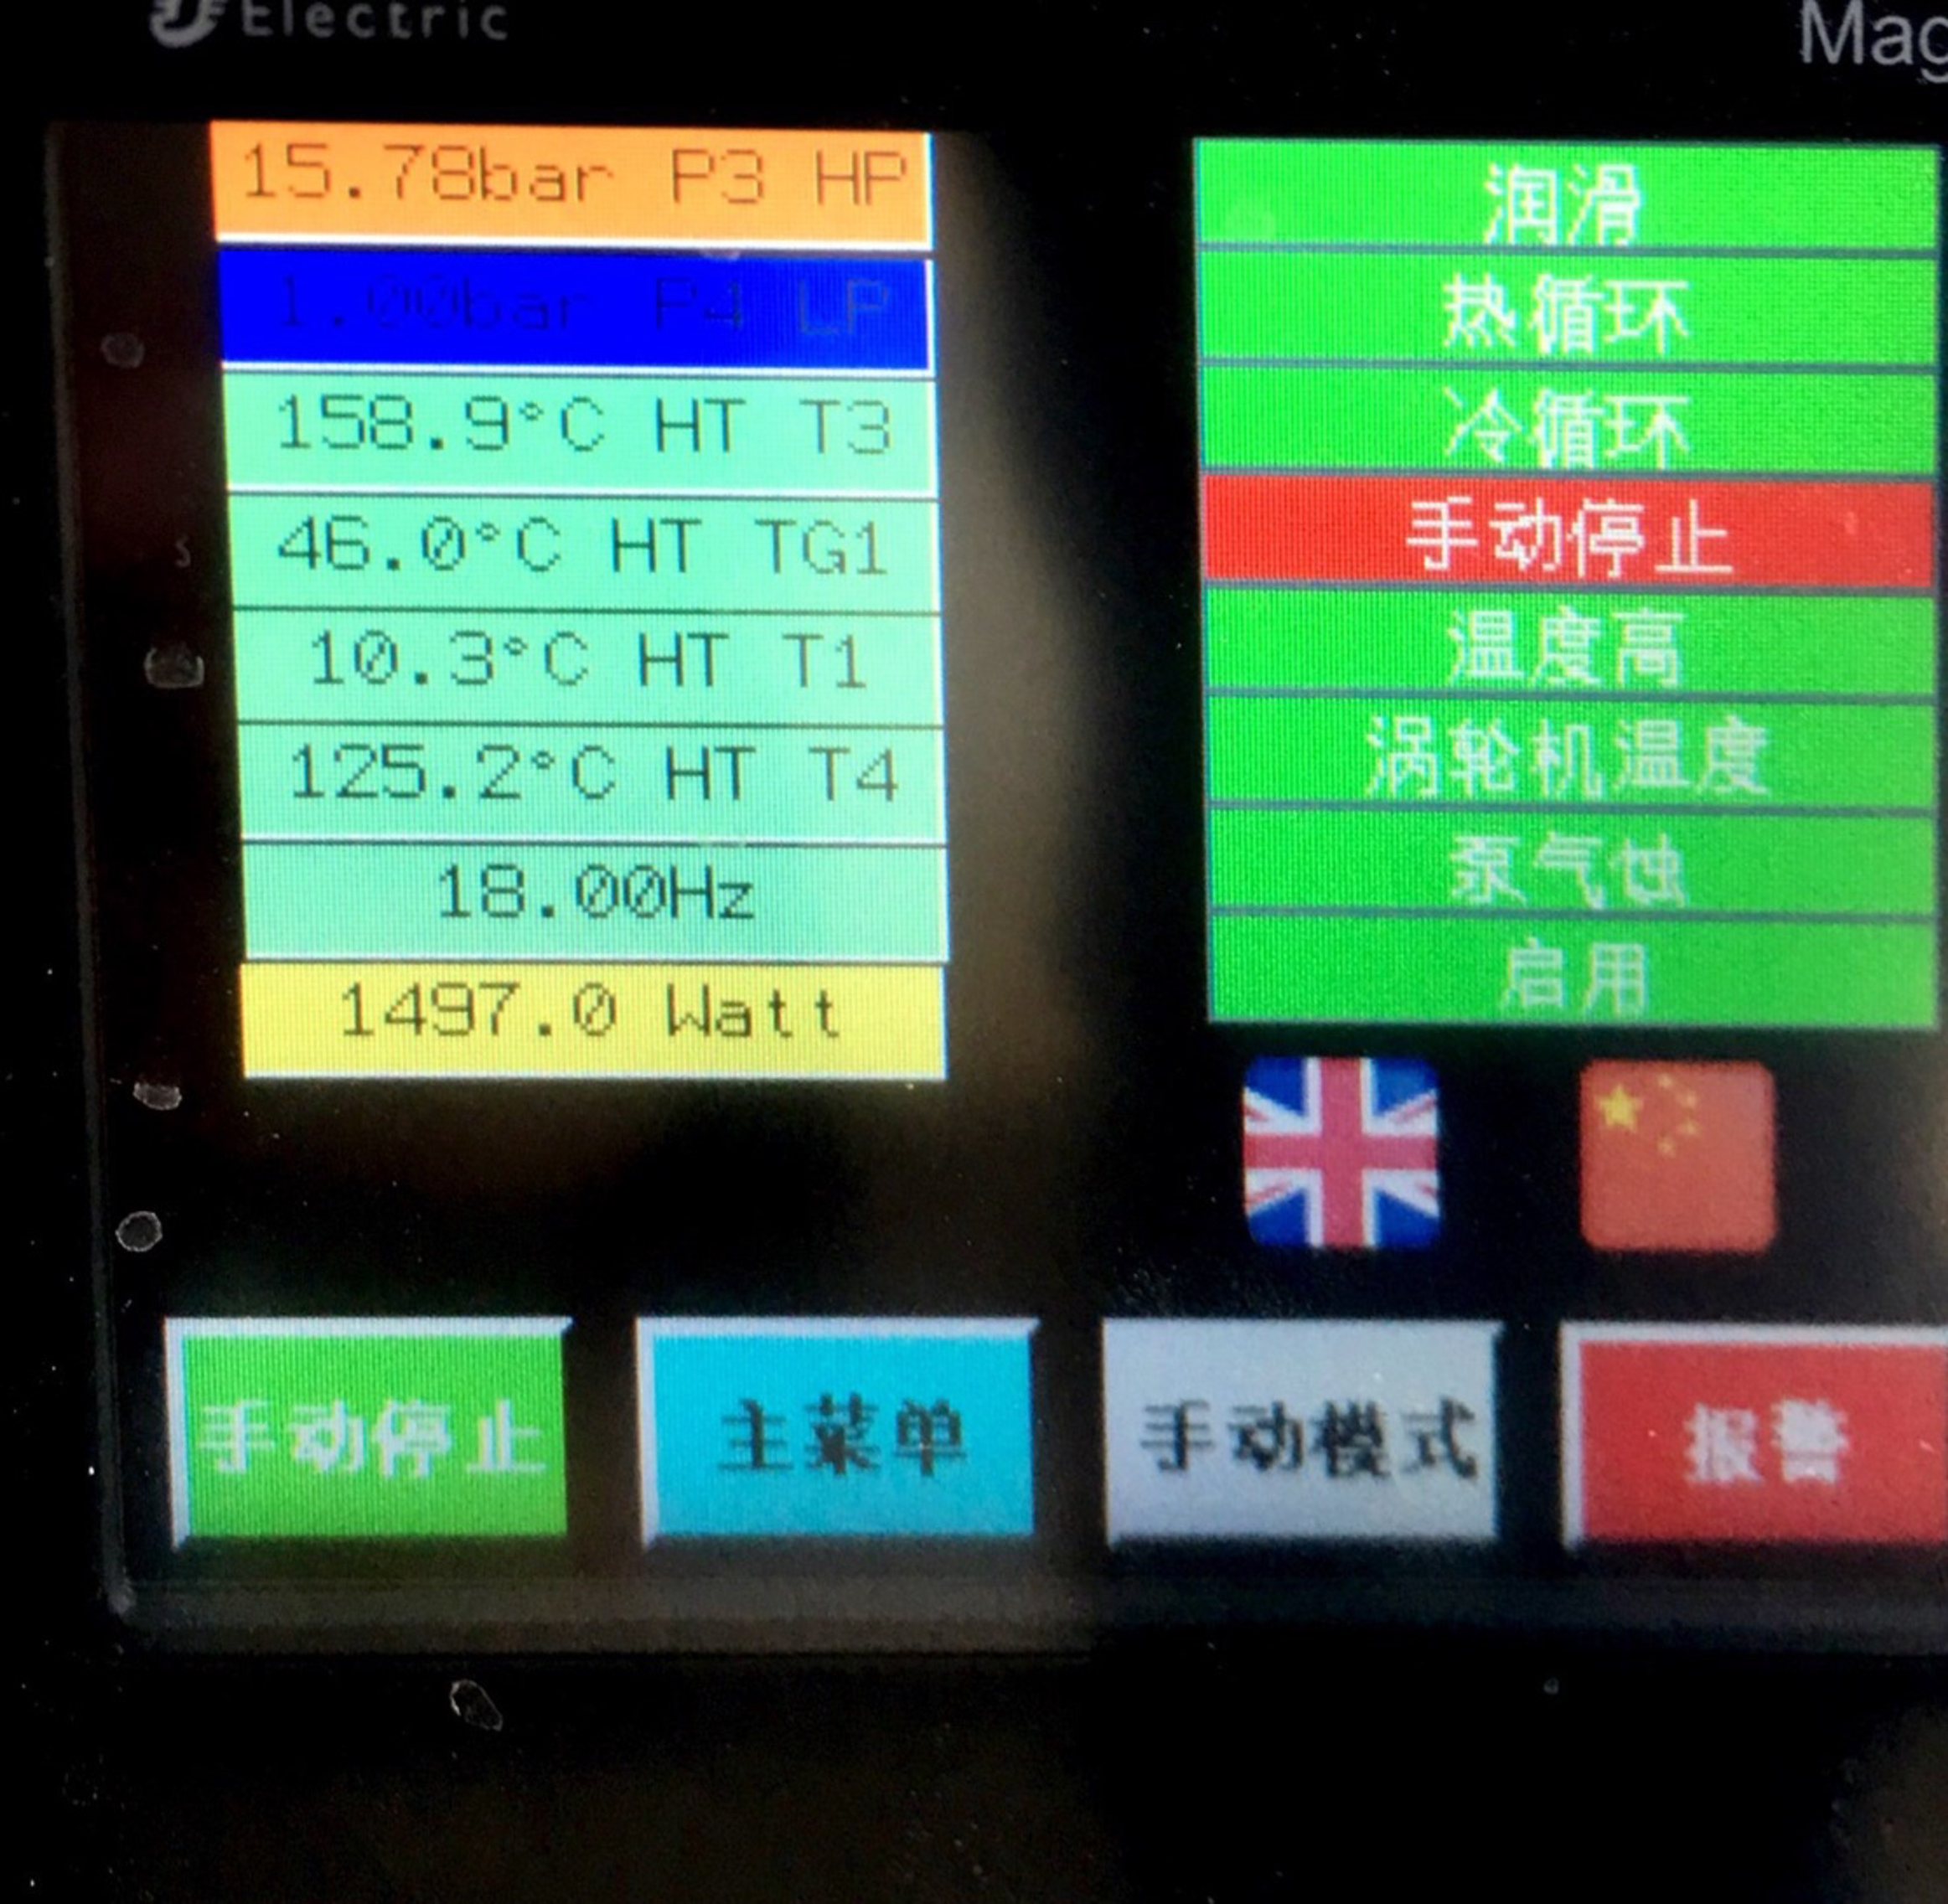
\includegraphics[width=0.4\textwidth]{fig/ControlCabinet}
\caption{Control screen of the ORC system}\label{fig:ControlCabinet}
\end{figure}

\subsection{Piping system}

Piping system provides the basis for fluid flow and heat exchange. Plus, it provides thermal insulation for hot fluids. Meters, pumps, valves, tanks and heaters are arranged in the piping system to maintain the normal and orderly operation.

Two heaters are used in the platform to increase the temperatures of the fluids (air and oil) to reach the experiment requirements when the solar irradiance is not enough. Both heaters have temperature sensors to maintain the temperatures of the outlet fluids by changing the power.
 

%\subsection{Data collection system}

\section{Experiments}

In order to test the performance of the platform and validate the proposed models, relevant experiments were carried out.
\subsection{Trough collector experiment}
\subsubsection{Experiment purpose}
The purpose of the experiment is to study the effects of solar irradiance, flow rate, inlet temperature of the working fluid on the thermal performance of the collector, and to validate the trough collector model established in section~\ref{sec:ptc}. 
\subsubsection{Experiment steps}
The operation steps are as follows,
\begin{enumerate}[label=(\arabic*)]
	\item Complete the preparation work. Ensure that the devices and components are all properly connected and can work normally.
	\item Initialize the solar radiometer. Adjust the direction of the solar radiometer to get the normal irradiation value, make sure the light spot passing through the tube falls in the designed position.
	\item Open the valves in the oil circuit, then turn on the oil pump.
	\item Turn on the motor of the trough collector tracking system. Synchronize the time of the tracking system, and turn on the automatic mode to make the trough system tracking the sun automatically.
	\item Adjust the parameters to meet the designed conditions. When the data is stable, record and save the data collected by the data acquisition system.
	\item Finish the experiment when all the design conditions have been tested.
	\item Rotate the trough collector to face towards the horizontal position on the control panel. Turn off the motor when the trough collector is ready in place.
	\item Turn off the oil pump.
\end{enumerate}

\subsubsection{Experiment cases}

%考虑到太阳直射辐射强度在晴天具有不可控性和相对连续性,当以太阳直射辐射强度为控制变量时,太阳辐射强度值不能控制为设计值,而应该为实测值。当需要固定太阳直射辐射强度时,应该尽量控制几组试验的总时间,减少太阳直射辐射强度变化带来的影响。

Considering the uncontrollability and continuity of the direct normal irradiance (DNI) in a clear day, when DNI is a control variable, solar irradiance values can not be controlled as design values and should be measured values. When DNI is required to be a constant, total experiment time should be limited to reduce the impact of DNI changes.

\begin{table}[htbp]\footnotesize
	\caption{Designed cases of the solar trough system}
	\begin{center}
	\begin{tabular}{cccc}
		\toprule
		Case	& DNI ($\mathrm{W/m^2}$)	&	Flow rate ($\mathrm{kg/s}$)			&	Inlet temperature ($\mathrm{K}$)\\
		\midrule
		1-9	&	Live values	&	0.20	&	433.2\\
		10	&	Live value	&	0.1	&	433.2\\
		11	&	Live value	&	0.2	&	433.2\\
		12	&	Live value	&	0.3	&	433.2\\
		13	&	Live value	&	0.4	&	433.2\\
		14	&	Live value	&	0.2	&	423.2\\
		15	&	Live value	&	0.2	&	433.2\\
		16	&	Live value	&	0.2	&	443.2\\
		17	&	Live value	&	0.2	&	453.2\\
		\bottomrule
	\end{tabular}
	\end{center}
	\label{tab:DesignedCasesForTrough}
\end{table}

In table~\ref{tab:DesignedCasesForTrough}, Case 1 to Case 9 are completed at different times of a day or in different days. Case 10 to Case 14 are required to be completed in half an hour. As the oil heating process takes more time, only 4 cases (Case 15 to Case 18) are designed for the inlet temperature investigation. And the 4 cases are required to be completed in an hour. It has to be noted that, the temperature range from Case 14 to Case 17 is small due to the slow heating process of the oil heater.

\subsubsection{Data processing method}
%Outlet temperature of the oil in the trough collector is monitored and recorded. 
The specific heat of the oil is given as: when $T = 373.15\mathrm{^\circ C}$, $c_p = 2.44\times10^3\,\mathrm{J/(kg\cdot K)}$; when $T = 473.15\mathrm{^\circ C}$, $c_p = 2.88\times10^3\,\mathrm{J/(kg\cdot K)}$. Linear interpolation method is applied, $c_p = aT + b$, where $a = 4.4\,\mathrm{J/(kg \cdot K^2)}$, $b = 798.14\,\mathrm{J/(kg\cdot K)}$.

The absorbed heat of the oil $Q_{abs} = \int_{T=T_i}^{T = T_o}c_p\dot{m}dT = \dfrac{1}{2}a(T_o^2 - T_i^2)\dot{m} + b (T_o - T_i)\dot{m}$.

The thermal efficiency of the trough collector 
\begin{equation}
	\eta_{tc} = \dfrac{Q_{abs}}{I_rw_{tc}L_{tc}}
	\label{eq:ExperimentEta}
\end{equation}

To validate the simulation model, Equation~\ref{eq:CTCHF} is required to be checked. In the simulation model,

\begin{equation}
	\widetilde{T_{o}}=T_{amb} + \dfrac{q''}{U(T_{abs})} + \exp(-\frac{U(T_{abs})\pi d_o L}{\dot{m}\widetilde{c_p}})(T_{i}-T_{amb}-\dfrac{q''}{U(T_{abs})})
	\label{eq:CheckT_o}
\end{equation}

where $T_{abs}$ is replaced by $(T_i + T_o)/2$ ($T_i$ and $T_o$ are the measured values of inlet temperature and outlet temperature), $\widetilde{c_p}$ is the average specific heat obtained from $(T_i + T_o)/2$,
$U(T_{abs})$ is obtained from~\cite{Romero2007}
\begin{equation}
	U(T_{abs}) = 0.687257 + 0.001941(T_{abs} - T_{amb}) + 0.000026(T_{abs} - T_{amb})^2
\end{equation}
\begin{equation}
	q'' = \frac{I_r w_{tc} \rho \gamma \tau F_e K(\theta)}{\pi d_o}
\end{equation}
\begin{equation}
	K(\theta) = \cos\theta+0.000884\theta-0.00005369\theta^2
\end{equation}

So $\widetilde{\eta_{tc}}$ from the simulation results can be obtained for comparison with the one in Equation~\ref{eq:ExperimentEta} obtained from experiment.
\begin{equation}
	\widetilde{\eta_{tc}} = \dfrac{\dot{m}\widetilde{c_p}(\widetilde{T_o}-T_i)}{I_rw_{tc}L_{tc}}
\end{equation}
	
\subsection{Dish collector experiment}
\subsubsection{Experiment purpose}
The purpose of the experiment is to study the effects of solar irradiance, flow rate, inlet temperature of the working fluid on the thermal performance of the collector, and to validate the dish receiver model established in section~\ref{sec:pdc}.

\subsubsection{Experiment steps}
 The operation steps are as follows,
\begin{enumerate}[label=(\arabic*)]
	\item Complete the preparation work. Ensure that the devices and components are all properly connected and can work normally.
	\item Initialize the solar radiometer. Adjust the direction of the solar radiometer to get the normal irradiation value, make sure the light spot passing through the tube falls in the designed position.
	\item Turn on the water cooling system.
	\item Open the valves of the inlet and outlet of the air circuit, then turn on the air compressor.
	\item Use manual mode to rotate the collector toward the sun. Then switch to the automative mode.
	\item Adjust the parameters to meet the designed conditions. When the data is stable, record and save the data collected by the data acquisition system.
	\item Finish the experiment when all the designed conditions have been tested. 
	\item Rotate the collector to the up most position (facing the zenith). Turn off the compressor, turn off the outlet and inlet valves, turn off the water cooling system.
\end{enumerate}

\subsubsection{Experiment cases}

\begin{table}[htbp]\footnotesize
	\caption{Designed cases of the solar dish system}
	\begin{center}
	\begin{tabular}{cccc}
		\toprule
		Case	& DNI ($\mathrm{W/m^2}$)	&	Flow rate ($\mathrm{kg/s}$)			&	Inlet temperature ($\mathrm{K}$)\\
		\midrule
		1-9	&	Live values	&	0.02	&	423.2\\
		10	&	Live value	&	0.01	&	423.2\\
		11	&	Live value	&	0.02	&	423.2\\
		12	&	Live value	&	0.03	&	423.2\\
		13	&	Live value	&	0.04	&	423.2\\
		14	&	Live value	&	0.02	&	373.2\\
		15	&	Live value	&	0.02	&	423.2\\
		16	&	Live value	&	0.02	&	473.2\\
		17	&	Live value	&	0.02	&	523.2\\
		\bottomrule
	\end{tabular}
	\end{center}
	\label{tab:DesignedCasesForDish}
\end{table}

In Table~\ref{tab:DesignedCasesForDish}, Case 1 to Case 9 are completed at different times of a day or in different days. Case 10 to Case 13 are required to be completed in half an hour. Case 15 to Case 18 are required to be completed in an hour.

\subsubsection{Data processing method}
Known the pressure ($p = 4\times10^5\,\mathrm{Pa}$) and the measured temperature, the inlet enthalpy ($h_i$) and outlet enthalpy ($h_o$) of the air can be obtained.

The absorbed heat of the air $Q_{abs} = \dot{m}(h_o - h_i)$.

The thermal efficiency of the dish collector $\eta_{dc} = \dfrac{Q_{abs}}{I_r A_{dc}}$. 

To validate the simulation model in section~\ref{sec:pdc}, %$T_{cav}$, $T_{insu}$ and $T_{amb}$ in the thermal network of dish receiver (see Figure~\ref{fig:thermal-lose}) are measured.
the thermal network of dish receiver (see Figure~\ref{fig:thermal-lose}) are solved from the equations in section~\ref{sec:pdc}.

The simulation efficiency of the dish collector $\widetilde{\eta_{dc}} = \dfrac{Q_{dr,1}}{I_r A_{dc}}$.

\section{Result analysis}
\subsection{Trough collector experiment result analysis}
Influences of solar irradiance, flow rate and inlet temperature of the working fluid on the collector thermal performance are concerned.
\subsubsection{Influence of $I_r$}
Tested values of Case 1 to Case 9 are listed in Table~\ref{tab:ResultOfTrough1}. It is noteworthy that due to the variability of solar radiation intensity, the measured values of solar irradiance are not evenly distributed.

\begin{table}[htbp]\footnotesize
	\caption{Experiment results of Case 1 to Case 9 of the trough collector}
	\begin{center}
	\begin{tabular}{cccccc}
		\toprule
		Case	& DNI ($\mathrm{W/m^2}$)	&	$\dot{m}$ ($\mathrm{kg/s}$)			&	$T_i$ ($\mathrm{K}$)	&	$T_o$ ($\mathrm{K}$)		&	$T_{amb}$ ($\mathrm{K}$)\\
		\midrule
		1	&	203	&	0.2	&	433.2	&	443.7	&	285.3\\
		2	&	258	&	0.2	&	433.2	&	446.8	&	284.2\\
		3	&	314	&	0.2	&	433.2	&	450.0	&	285.4	\\
		4	&	326	&	0.2	&	433.2	&	450.6	&	286.8\\
		5	&	347	&	0.2	&	433.2	&	451.8	&	293.7\\
		6	&	358	&	0.2	&	433.2	&	452.4	&	287.5\\
		7	&	403	&	0.2	&	433.2	&	455.0	&	289.5\\
		8	&	460	&	0.2	&	433.2	&	458.2	&	289.3\\
		9	&	487	&	0.2	&	433.2	&	459.7	&	296.6\\
		\bottomrule
	\end{tabular}
	\end{center}
	\label{tab:ResultOfTrough1}
\end{table}

Figure~\ref{fig:I_r-eta-trough} shows the influence of solar irradiance on the thermal efficiency of the trough collector. Curve of simulation result is also included. The simulation parameters are set to be the same as the experiment. 
%The optical efficiency fo the dish collector is manually reduced to simulate the real situation of the spilled focused spot.
\begin{figure}[!ht]
\centering
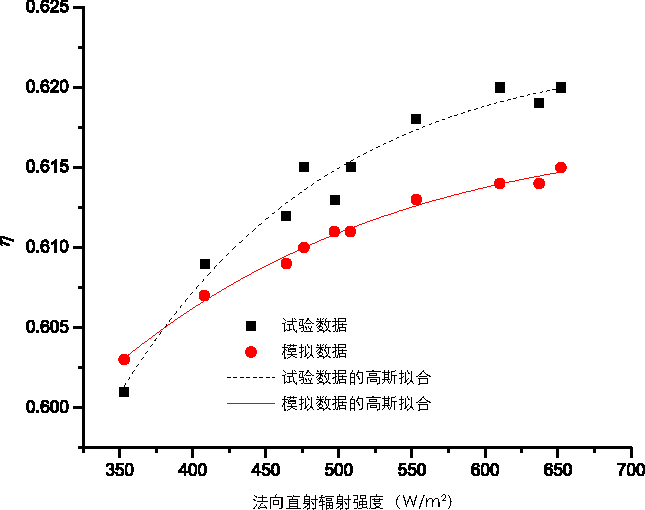
\includegraphics[width=0.7\textwidth]{fig/I_r-eta-trough}
\caption{Influence of solar irradiance on the thermal efficiency}
\label{fig:I_r-eta-trough}
\end{figure}

It can be found that both the experiment data and simulation result show the same trend of thermal efficiency and solar irradiance. Bumps on the fit curve may be interpreted as the effect of ambient temperature. As shown in Table~\ref{tab:ResultOfTrough1}, the ambient temperature of Case 5 (293.7$\,\mathrm{K}$) is significantly higher than that of other cases, which helps for higher thermal efficiency.

\subsubsection{Influence of $\dot{m}$}
Tested values of Case 10 to Case 13 are listed in Table~\ref{tab:ResultOfTrough2}.

\begin{table}[htbp]\footnotesize
	\caption{Experiment results of Case 10 to Case 13 of the trough collector}
	\begin{center}
	\begin{tabular}{cccccc}
		\toprule
		Case	& DNI ($\mathrm{W/m^2}$)	&	$\dot{m}$ ($\mathrm{kg/s}$)			&	$T_i$ ($\mathrm{K}$)	&	$T_o$ ($\mathrm{K}$)		&	$T_{amb}$ ($\mathrm{K}$)\\
		\midrule
		10	&	348	&	0.1	&	433.2	&	466.7	&	289.3\\
		11	&	349	&	0.2	&	433.2	&	450.8	&	289.3\\
		12	&	351	&	0.3	&	433.2	&	445.2	&	289.4	\\
		13	&	354	&	0.4	&	433.2	&	442.3	&	290.0\\
		\bottomrule
	\end{tabular}
	\end{center}
	\label{tab:ResultOfTrough2}
\end{table}

Figure~\ref{fig:q_m-eta-trough} shows the influence of inlet flow rate on the thermal efficiency of the dish collector. The data points in the figure are collected in a short time, so the irradiance can be regarded as unchanged.
\begin{figure}[!ht]
\centering
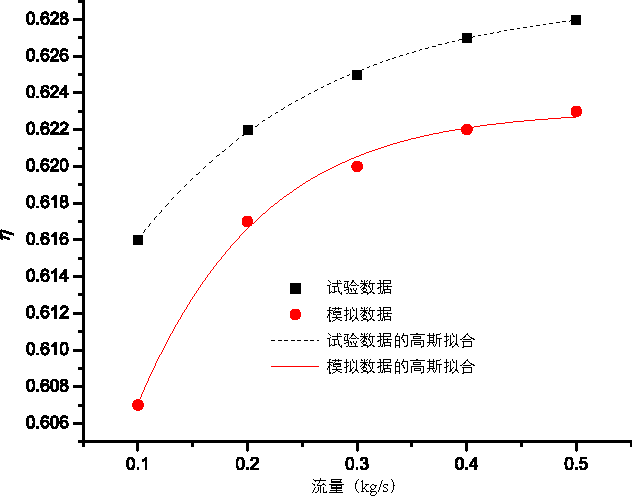
\includegraphics[width=0.7\textwidth]{fig/q_m-eta-trough}
\caption{Influence of inlet flow rate on the thermal efficiency}
\label{fig:q_m-eta-trough}
\end{figure}

It can be found that higher flow rate leads to higher efficiency. This is obvious for higher flow rate takes more heat from the receiver, leads to lower temperature distribution and hence less thermal losses. The experimental data and simulation result are in good agreement.

\subsubsection{Influence of $T_i$}
Tested values of Case 14 to Case 17 are listed in Table~\ref{tab:ResultOfDish3}.

\begin{table}[htbp]\footnotesize
	\caption{Experiment results of Case 14 to Case 17 of the trough collector}
	\begin{center}
	\begin{tabular}{cccccc}
		\toprule
		Case	& DNI ($\mathrm{W/m^2}$)	&	$\dot{m}$ ($\mathrm{kg/s}$)			&	$T_i$ ($\mathrm{K}$)	&	$T_o$ ($\mathrm{K}$)		&	$T_{amb}$ ($\mathrm{K}$)\\
		\midrule
		14	&	355	&	0.07	&	373.2	&	452.2	&	290.0\\
		15	&	356	&	0.07	&	423.2	&	500.7	&	290.1\\
		16	&	358	&	0.07	&	473.2	&	548.3	&	290.2	\\
		17	&	361	&	0.07	&	523.2	&	596.0	&	290.2\\
		\bottomrule
	\end{tabular}
	\end{center}
	\label{tab:ResultOfDish3}
\end{table}

Figure~\ref{fig:T_i-eta-trough} shows the influence of inlet flow rate on the thermal efficiency of the trough collector.
\begin{figure}[!ht]
\centering
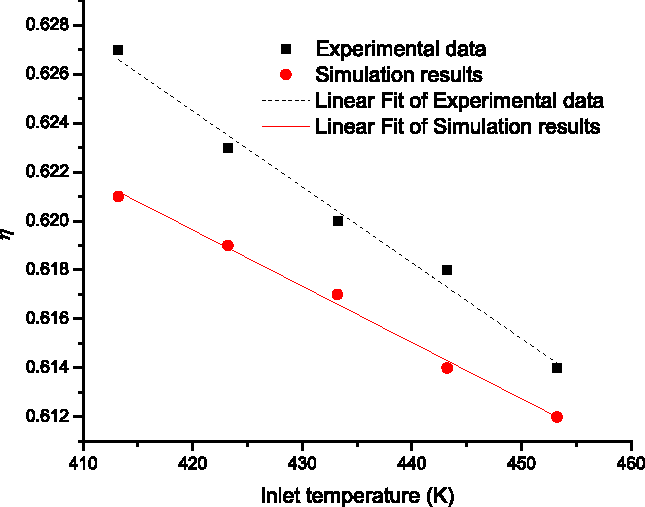
\includegraphics[width=0.7\textwidth]{fig/T_i-eta-trough}
\caption{Influence of inlet temperature on the thermal efficiency}
\label{fig:T_i-eta-trough}
\end{figure}

It can be found that higher inlet temperature leads to lower efficiency, This is obvious for higher inlet temperature leads to higher temperature distribution and hence more thermal losses. The experimental data and simulation result are in good agreement.

\subsection{Dish collector experiment result analysis}
Influences of solar irradiance, flow rate and inlet temperature of the working fluid on the collector thermal performance are concerned.
\subsubsection{Influence of $I_r$}
Tested values of Case 1 to Case 9 are listed in Table~\ref{tab:ResultOfDish1}. It is noteworthy that due to the variability of solar radiation intensity, the measured values of solar irradiance are not evenly distributed.

\begin{table}[htbp]\footnotesize
	\caption{Experiment results of Case 1 to Case 9 of the dish collector}
	\begin{center}
	\begin{tabular}{cccccc}
		\toprule
		Case	& DNI ($\mathrm{W/m^2}$)	&	$\dot{m}$ ($\mathrm{kg/s}$)			&	$T_i$ ($\mathrm{K}$)	&	$T_o$ ($\mathrm{K}$)		&	$T_{amb}$ ($\mathrm{K}$)\\
		\midrule
		1	&	203	&	0.04	&	423.2	&	466.7	&	285.3\\
		2	&	258	&	0.04	&	423.2	&	478.6	&	284.2\\
		3	&	314	&	0.04	&	423.2	&	491.8	&	285.4	\\
		4	&	326	&	0.04	&	423.2	&	494.8	&	286.8\\
		5	&	347	&	0.04	&	423.2	&	498.3	&	293.7\\
		6	&	358	&	0.04	&	423.2	&	500.8	&	287.5\\
		7	&	403	&	0.04	&	423.2	&	510.9	&	289.5\\
		8	&	460	&	0.04	&	423.2	&	523.5	&	289.3\\
		9	&	487	&	0.04	&	423.2	&	529.5	&	296.6\\
		\bottomrule
	\end{tabular}
	\end{center}
	\label{tab:ResultOfDish1}
\end{table}

Figure~\ref{fig:I_r-eta} shows the influence of solar irradiance on the thermal efficiency of the dish collector. Curve of simulation result is also included. The simulation parameters are set to be the same as the experiment. 
%The optical efficiency fo the dish collector is manually reduced to simulate the real situation of the spilled focused spot.
\begin{figure}[!ht]
\centering
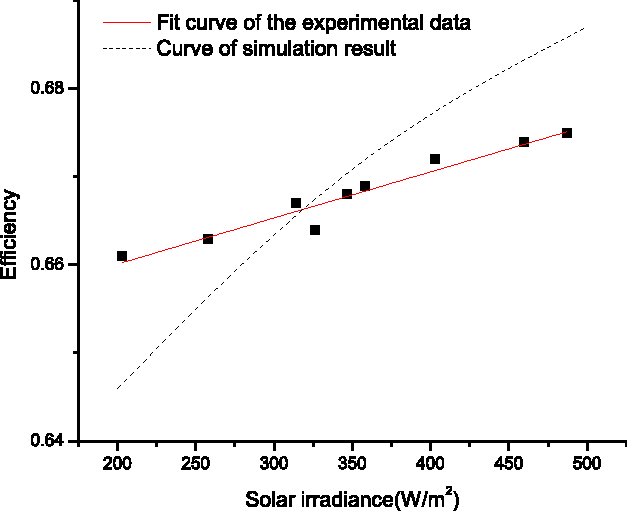
\includegraphics[width=0.7\textwidth]{fig/I_r-eta}
\caption{Influence of solar irradiance on the thermal efficiency}
\label{fig:I_r-eta}
\end{figure}

It can be found that the thermal efficiency has little increment while the solar irradiance increased from 200$\,\mathrm{W/m}^2$ to 500$\,\mathrm{W/m}^2$, which has the same trends with theoretical model. With the increment of solar irradiance, more energy is injected into the receiver. The temperatures of the entrance section of the pipe, and the outer wall are not increased obviously. So the increasing amount of heat loss is not so much compared with the increased input energy. 
The discrepancy of the experimental data and simulation data may be interpreted for the insulation condition. The higher out wall temperature of the insulation layer shows that the isolation condition is not good enough. Higher irradiance leads to higher wall temperature and hence more radiation loss, which jeopardizes the thermal efficiency when solar irradiance increases.

%However, it has to be pointed out that these data points were collected in different days, the environment temperature and wind speed may differ. It needs further researches on this topic.

\subsubsection{Influence of $\dot{m}$}

Tested values of Case 10 to Case 13 are listed in Table~\ref{tab:ResultOfDish2}.

\begin{table}[htbp]\footnotesize
	\caption{Experiment results of Case 10 to Case 13 of the dish collector}
	\begin{center}
	\begin{tabular}{cccccc}
		\toprule
		Case	& DNI ($\mathrm{W/m^2}$)	&	$\dot{m}$ ($\mathrm{kg/s}$)			&	$T_i$ ($\mathrm{K}$)	&	$T_o$ ($\mathrm{K}$)		&	$T_{amb}$ ($\mathrm{K}$)\\
		\midrule
		10	&	348	&	0.05	&	423.2	&	527.4	&	289.3\\
		11	&	349	&	0.07	&	423.2	&	498.2	&	289.3\\
		12	&	351	&	0.09	&	423.2	&	482.8	&	289.4	\\
		13	&	354	&	0.11	&	423.2	&	472.7	&	290.0\\
		\bottomrule
	\end{tabular}
	\end{center}
	\label{tab:ResultOfDish2}
\end{table}


Figure~\ref{fig:q_m-eta} shows the influence of inlet flow rate on the thermal efficiency of the dish collector. The data points in the figure are collected in a short time, so the irradiance can be regarded as unchanged.
\begin{figure}[!ht]
\centering
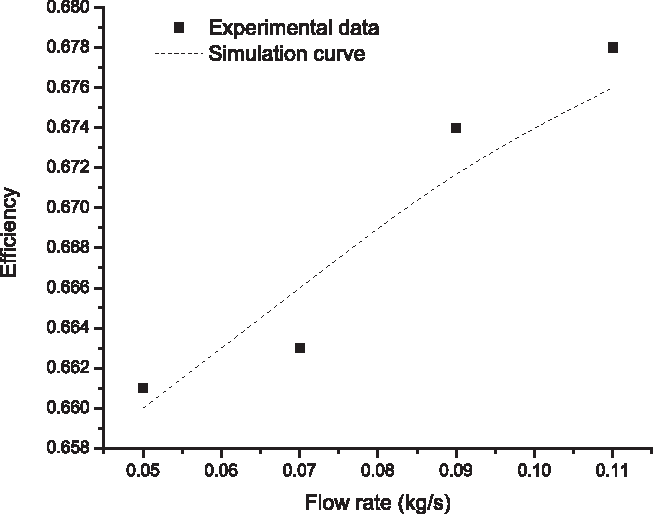
\includegraphics[width=0.7\textwidth]{fig/q_m-eta}
\caption{Influence of inlet flow rate on the thermal efficiency}
\label{fig:q_m-eta}
\end{figure}

It can be found that higher flow rate leads to higher efficiency. This is obvious for higher flow rate takes more heat from the receiver, leads to lower temperature distribution and hence less thermal losses. The experimental data and simulation result are in good agreement.

\subsubsection{Influence of $T_i$}

Tested values of Case 14 to Case 17 are listed in Table~\ref{tab:ResultOfDish3}.

\begin{table}[htbp]\footnotesize
	\caption{Experiment results of Case 14 to Case 17 of the dish collector}
	\begin{center}
	\begin{tabular}{cccccc}
		\toprule
		Case	& DNI ($\mathrm{W/m^2}$)	&	$\dot{m}$ ($\mathrm{kg/s}$)			&	$T_i$ ($\mathrm{K}$)	&	$T_o$ ($\mathrm{K}$)		&	$T_{amb}$ ($\mathrm{K}$)\\
		\midrule
		14	&	355	&	0.07	&	373.2	&	452.2	&	290.0\\
		15	&	356	&	0.07	&	423.2	&	500.7	&	290.1\\
		16	&	358	&	0.07	&	473.2	&	548.3	&	290.2	\\
		17	&	361	&	0.07	&	523.2	&	596.0	&	290.2\\
		\bottomrule
	\end{tabular}
	\end{center}
	\label{tab:ResultOfDish3}
\end{table}

Figure~\ref{fig:T_i-eta} shows the influence of inlet flow rate on the thermal efficiency of the dish collector.
\begin{figure}[!ht]
\centering
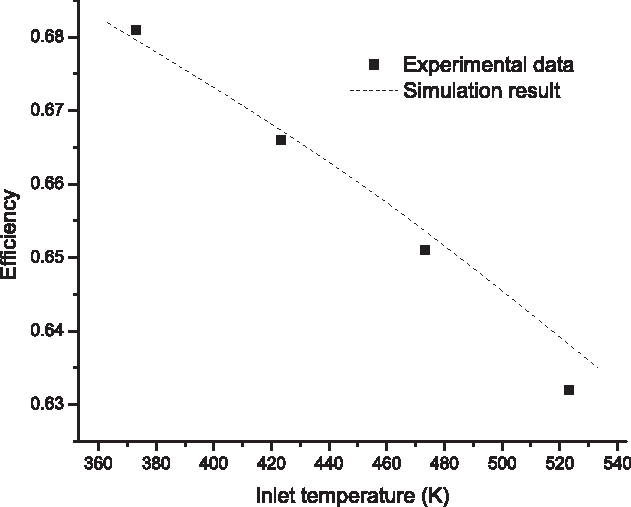
\includegraphics[width=0.7\textwidth]{fig/T_i-eta}
\caption{Influence of inlet temperature on the thermal efficiency}
\label{fig:T_i-eta}
\end{figure}

It can be found that higher inlet temperature leads to lower efficiency, This is obvious for higher inlet temperature leads to higher temperature distribution and hence more thermal losses. The experimental data and simulation result are in good agreement.

\section{Conclusion}
The solar thermal power platform is a good start for the cascade solar thermal system.
Experiment results

The thermal efficiency of trough collectors is between 58\% and 64\% and the thermal efficiency of dish collectors is between 63\% and 68\%.